\chapter{Discussion}

\section{Super servers}

The functionality developed in this thesis is commonly referred to as a \emph{super server}.
A super server is a program which orchestrates communication with multiple service implementations on a single computer, e.g. handling a daemon for the FTP protocol as well as another daemon providing time via NTP.

Super servers have initially been designed with the overarching goal of resource conservation in mind.
Instead of starting up all service daemons at system boot time, only the super server daemon in started up at system boot.
It will then bind to configured ports and listen for incoming connections.
As soon as a client connects then, the actual service executable will be started on demand and given access to the client's socket.

The first super server has been the so-called internet daemon \emph{inetd}, which has been initially released with 4.3BSD in 1986 \cite{inetd}.
inetd is set up by writing a simple configuration file specifying all services that should be supervised by the daemon.
Each service can be configured by providing multiple parameters, like socket type, protocol, which user it shall execute as and the actual command that shall be executed when a connection is received.

The initial implementation only provided this basic functionality.
Most importantly, there was no mechanism for access control as well as no rate limiting available.
To fix these shortcomings, Panagiotis Tsirigotis started work on the \emph{extended internet daemon} xinetd in 1992 \cite{xinetd}, which in contrast to inetd also contains basic rate limiting as well as access control by using \emph{tcp-wrappers}.
tcp-wrappers \cite{venema1992tcp} is a simple tool which allows to black- or whitelist access by using network addresses.
It furthermore provides the ability to log connections to be able to monitor what is going on on a server.

Rate limiting may be configured via three different parameters: overall rate of connections received, rate of connections received for a single service as well as connections received from a specific IP address.
These parameters may all be configured independently of each other to throttle overall resource usage or to throttle single clients.

The access control mechanisms employed are rather simplistic.
Rather than providing authentication by a user's identity, all authentication is solved by inspecting IP addresses.
That is for each service, one can define white- as well as blacklists detailing which IP address or range of IP addresses may access the service and which may not.
So in order to guarantee working access control, network administrators need to make sure that clients have fixed IP addresses as otherwise it is easily possible to access services by changing a computers IP address.

Another implementation for a super server is \emph{ucspi-tcp} by D.J. Bernstein \cite{ucspi-tcp}.
ucspi-tcp has been developed in the early 1990s, as well, with an initial alpha being released in 1996.
It was intended as a replacement for the inetd daemon, trying to solve several problems encountered with it.

The main grieves of Bernstein was that inetd was unreliable under higher loads, inetd simply cut off service when it received too many connections in a short amount of time \cite{ucspi-tcp}.
Furthermore, it did also happily consume all resources of the system when many services are started at the same time.
To help those cases, ucspi-tcp went down the same route as xinetd by introducing rate limiting.

One additional feature implemented by ucspi-tcp was authentication via the IDENT protocol.
ucspi-tcp might require authentication of users by having them sign in to user accounts local to the machine the executable runs on.
This has also been employed later on by inetd and xinetd.

\bigskip

Comparing the above implementations of super servers to our implementation, there are three observations to be made:

\emph{First}, it is of importance to provide mechanisms to limit resource utilization.
As it seems, a big grief with initial implementations of inetd were that it was not possible to have proper rate limiting and thus protect the resources of servers that it runs on.
The current implementation in this thesis does not provide any means of rate limiting connections.
Due to timing constraints, it was not possible to implement this feature.

\emph{Second}, none of the listed implementations is ``secure by default'':
In contrast to our approach where all connections between client and service are tunneled through an encrypted channel, these super servers simply start up the service and let it subsequently perform its protocol, relying on security measurements of the protocol's implementation.

This probably results from the fact that the initial scenario for which these solutions have been developed is to tackle resource scarcity problems on the server side.
Security has not been a consideration up front.

\emph{Third}, authentication, if available at all, is either based on IP addresses or centrally managed user accounts.
The first case of authentication through IP addresses seems at best unfortunate.
Considering our adversary's abilities of reading and injecting messages at will while spoofing network addresses, this obviously does not suffice to efficiently protect a service.

Using centrally managed user accounts is roughly equivalent to managing user's public keys on a server.
In contrast to user accounts, though, our approach based on capabilities allows more flexibility by granting other users the ability to execute services which they normally would not have the rights to do so, if the capability is created by another known identity by having other entities generate and pass on capabilities.

To the best of our knowledge, no other super server currently exists covering the concrete use case envisioned in this thesis, namely having a secure-by-default protocol which allows for easy passing on of access rights controllable by a third entity.

\section{Service discovery}

The thesis does include a mechanism to discover services using a custom protocol based on Googles Protocol Buffers.
The actual implementation is a very simple one, only providing peer-to-peer service discovery in the local network:
Given a client which wants to discover all services present in the local network, it will simply send a query to the broadcast address and await announces by available servers.

The service discovery part of this thesis is only provided to get a fully-working proof of concept, providing all steps required to achieve the goal of connecting distributed resources.
As such, the main focus is \emph{not} on the service discovery protocol and the complete discovery process may be exchanged as the framework matures in favor of a different, already established protocol.
Nevertheless, we will investigate some of the implications and requirements based on our use case.

There exist many different protocols used for device discovery, where most protocols have a special focus which is mandated by the actual field of application it has been designed for.
E.g. service discovery in enterprises where centralized infrastructure exists will usually be implemented in a different way to service discovery in a distributed environment.
In \cite{zhu2005service}, a set of ten aspects has been developed which aim to categorize discovery protocols, where we will now discuss a subset of these aspects.

The \emph{initial communication method} states how a peer will gain knowledge about available services when it wants to connect to a network.
There are three major cases with unicast, multicast and broadcast.
Unicast is usable only when a centralized architecture is given, e.g. in the case of a directory service (DS) which is already known to all peers.
The peer will connect to the DS and ask it to provide all services having registered with the DS.
Obviously, unicast solutions are not going to work in our generalized use case of distributed resources, where clients might not have prior knowledge of DS's.

In settings where the network infrastructure is unknown, clients may use either multicast or broadcast to get knowledge of services.
When using multicast, a client will initially broadcast messages into the network, receiving announcements from available services.
Based on these announcements, the client will switch to unicast messages directed towards these services.
Broadcast-based protocols instead completely rely on link-layer broadcast messages without any direct connection to services.
The main benefit of using multicast- over broadcast-based protocols is reduced network bandwidth \cite{zhu2005service,edwards2006discovery}.

Our service discovery implementation uses multicast to support device discovery in distributed networks.
Initially, a discovery request is sent to the special multicast address \lstinline{224.0.0.1}, which will cause the message to be distributed to all hosts on the same network segment.
All listening servers can now respond with a list of services they provide.
Following initial service discovery, the client may now send unicast messages to these servers to either update the list of services they provide or to get further knowledge about one of these services.
When new servers connect to the network, there are currently no notifications sent by these servers to clients.
It results that clients have to poll the network when they want to discover newly connected servers.

To lessen the strains on the network, we have employed the multicast convergence algorithm used in the Service Location Protocol (SLP) \cite{guttman1999service}.
The SLP multicast convergence algorithm simply adds all servers already known to the client to the initial multicast message.
When a server receives this message, it will check if the client already has knowledge of the server and, if so, will not announce its availability again.
Like this, only previously unknown servers will announce their availability to the peer.

The \emph{service discovery infrastructure} criterion draws a distinction between systems based on directories and pure peer-to-peer protocols without any sort of directories.
Directory-based protocols require special hosts which keep track of all servers which provide any services to the domain.
When a client wants to get to know all services in this domain, it is enough for it to simply discover the directory service and then ask it for all services.

Our protocol instead uses a simple peer-to-peer system without any sort of directories.
While this works for small network environments like a home network, this approach is hard to scale up due to the induced network link strain.

Some systems exist which try to handle both scenarios at once by using a hybrid approach, with SLP being one of these systems.
Optional directory agents might be deployed into the network which listen to service announcements and add them to a list of known services.
When a client now connects to the network, it will initially try to discover if any directory agents are present and, if so, from now on use them to discover services.
Especially when considering the setting of Intern of Things, where a plethora of devices might be present, this is mode of operation becomes interesting.

Of special interest to us is the support of \emph{discovery scopes}.
While many protocols, including the proof of concept one employed by us, are only able to handle a scope based on the network topology, some have additional scoping features.
One of these protocols is the Ninja Service Discovery Service \cite{czerwinski1999architecture} by Czerwinski et al.
Besides supporting network topology service discovery, they also support context-aware (e.g. all devices in the current room) as well as user role based service discovery.

User role based service discovery becomes of special interest when combined with service privacy, like it is done in the Ninja SDS.
Given this combination of features, it is possible to restrict announced services based on the peer's identity.
Like this it becomes possible to provide discovery for services which shall not be publicly known to be available but instead only for peers with a certain clearance level.

User role based access control obviously relies on the availability of information on data authenticating users to the discovery service.
Due to this fact, this feature is almost only available to directory-based service discovery protocols with centralized infrastructure, as is the case for the Ninja SDS.
To the best of our knowledge, Universal Plug and Play (UPnP) \cite{miller2001home}, which uses the Simple Service Discovery Protocol (SSDP), is the only widely used protocol which uses a peer-to-peer architecture and at the same time performs authentication and authorization of its peers via access control lists \cite{zhu2005service,edwards2006discovery}.
Unfortunately, authentication and authorization is only available in the form of extensions of SSDP (e.g.  in \cite{ellison2003device}) and is not widely used.
Furthermore, no service confidentiality is granted like it is done for Ninja.

\bigskip

The current service discovery implementation is only intended as a proof of concept for this thesis.
Summarizing our findings, especially support for directories is required when trying to scale up, as well as missing access control.

Instead of reinventing the wheel, one might consider integrating the service architecture into existing solutions.
Currently, no perfect solution exists which is able to handle peer-to-peer discovery as well as directory discovery while also providing the ability to do authentication, authorization and access control for peers.

One of the more interesting protocols for centralized service discovery is the Ninja SDS, as it provides many security-related features as well as service confidentiality.
Regarding flexibility, SLP is another interesting protocol which is able perform peer-to-peer discovery, but to also scale up in the presence of directory agents.
A solution borrowing features from both protocols might be sufficient to solve most of our desired features.

\section{Key exchange}
\label{sec:key-exchange}

The initial step of all direct connections between client and server is the key exchange, where a shared secret is generated which will subsequently be used to encrypt all communication.
As the protocol is designed to be usable in a decentralized environment, no central key distribution center exists which aids in this process.
Instead, all keys shall be derived using the long-term signature keys of both client and server.
The shared secret that is generated should have the property that it is not derivable by a third party while being able to determine that the key can only be derived with the party that we intend to communicate with.
Our implementation only considers key exchange between two participants, as there are never more than two parties directly communicating with each other inside the same session.

A requirement of the actual key exchange protocol is that it has to match our security model outlined in our problem definition.
The adversary has the ability to modify all network traffic and spoofing network addresses for all participants of the protocol.
In order to have a secure key exchange under this model, the chosen protocol has to be secure under either this exact model or a model where the adversary has even more power.

When exchanging a key between two entities, one can distinguish between \emph{key transport} and \emph{key agreement} protocols \cite{menezes1996handbook}.
Key transport protocols involve one entity creating a secret which is then shared with a second entity.
Key agreement protocols derive a key by using information contributed by both parties such that no party is able to force a desired key.
The generated key is usually called a \emph{session key}.

In our protocol, we have chosen to perform the initial key exchange via an key agreement protocol based on long-term signature keys.
Each identity has a key pair, where the public key is assumed to be known to other parties wishing to share a secret.
As all actions are heavily bound to these keys in that all access control is based on the public long-term signature key of associated entities, we have a strong requirement for authentication.
So the initial connection establishment performs a form of authenticated key agreement (AK).

In order to guarantee authenticity as well as achieve confirmation of the identity of the remote party we are performing AK with, two properties need to be fulfilled \cite{law2003efficient}.
Implicit key authentication is given when one participant of the protocol can be assured that no other entity than the intended recipient is able to get to know a specific secret.
Key confirmation is given when one participant of the protocol can be assured that the other participant actually \emph{has} knowledge of a specific secret.
Authenticated key agreement protocols which have both implicit key authentication as well as key confirmation are called an emph{authenticated key agreement protocols with key confirmation} (AKC).

There exist five properties that are commonly cited when analyzing AK or AKC protocols \cite{menezes1996handbook,blake1997key,law2003efficient}:
\begin{enumerate}
    \item \emph{known-key security}
        If session keys have been compromised, the adversary is not able to impact secrecy of the protocol.
    \item \emph{(perfect) forward secrecy}
        If a long-term signature key gets compromised, the adversary is not able to impact secrecy of previous session keys.
    \item \emph{key-compromise impersonation}
        If a long-term signature key of an entity has been compromised, the adversary is not able to impersonate other entities towards the entity whom the key has been stolen from.
    \item \emph{unknown key-share}
        An adversary is not able to coerce an entity A to share a new secret key with another entity B without knowledge of entity A.
    \item \emph{key control}
        No entity is able to force the session key to a pre-determined secret.
\end{enumerate}
There exist several protocols which fulfill all these criteria.

Blake-Wilson et al. propose multiple protocols for AK as well as AKC \cite{blake1997key}.
All these schemes are based upon the Diffie-Hellman problem \cite{diffie1976new}.
They assume an adversary who is able control communication between all entities and able to ask entities at any time to reveal their long-term signature keys.
In their model, an AK or AKC model is secure if no adversary is able to learn anything about a session key held between two uncompromised entities (that is an entity whose long-term signature key has not been revealed).

Even given this powerful adversary, Blake-Wilson is able to come up with a provably secure scheme for AK and AKC, assuming the underlying cryptographic primitives are secure.
Two protocols are of further interest to this thesis, as they describe an AKC protocol based on public-key cryptography.
Unfortunately, though, these protocols require a long-term established secret between both parties, which makes it unsuitable for highly distributed scenarios.

In \cite{canetti2001analysis}, Canetty and Krawczyk propose the SIG-DH protocol, an AKC protocol usable with any digital signature scheme.
It is essentially a three-pass protocol based upon the Diffie-Hellman problem and public key signatures with added key confirmation.

The protocol is proven to be secure in the unauthenticated links model (UM).
In the UM, the adversary ``\emph{can listen to all the transmitted information, decide what messages will reach their destination and when, change these messages at will or inject its own generated messages. [\ldots] In addition to these basic adversarial capabilities [\ldots], we let the attacker obtain secret information stored in the parties memories via explicit attacks.}'' \cite{canetti2001analysis}.
The adversary is able to reveal the current session-state, the session's ephemeral key as well as all secret memory like long-term secrets.

Obviously, the UM's adversary is much stronger than the adversary we have assumed, which is only able to control the network and not able of revealing any secret state held.
As SIG-DH is proven secure in the stronger UM, it will hold secure in our model with a weaker adversary.

In \cite{lamacchia2007stronger}, LaMacchia et al. have shown a weakness in the SIG-DH protocol when using a non-deterministic signature scheme:
\begin{quote}
    For randomized signature schemes such as ElGamal, Schnorr, DSA and QG there exists an efficient algorithm which given a public key, a legitimately computed signature of any message (under the corresponding secret key) and random coins used by a signer, computes the secret key. \cite{lamacchia2007stronger}
\end{quote}
So an adversary may attack SIG-DH by initiating a new session between two parties and recording public keys as well as the signatures generated, revealing the random coins used to generate them.
Like this the attacker is able to determine the party's long-term signature key.

Despite the fact that the protocol is vulnerable for non-deterministic signature schemes, we have chosen it as the AKC used in our protocol.
The main reason for this is its proven security as well as that it does not require any previously shared state between the two parties wishing to generate a shared secret with each other, like it is required for other protocols like e.g. the ones proposed by Blake-Wilson.
In order to not fall for the protocol's weakness, we use the signature scheme Ed25519 developed by Bernstein et al. \cite{bernstein2012high}, which is a deterministic signature scheme, rendering it invulnerable to the attack by LaMacchia.

\bigskip

The AKC protocol handles the process of key derival in an authorized way.
What it does not solve though is the problem of attaining access to the actual long-term public signature keys themselves.
That is given two entities who are previously unknown to each other, we want them to exchange their long-term public signature keys in a secure way.
While this problem is explicitly \emph{not} in scope for this thesis, we will briefly discuss the subject.
All following schemes are just examples of how the problem may be solved without actually judging these schemes one by one.

When two parties whose identities are previously unknown to each other, it is trivial for an adversary to intercept all communication and pretend to be the other identity, as both parties have no way to actually verify whom they are talking to.
As such, it is obvious that some kind of side-channel needs to exist in order to help the case.

In the case of two actual users who mutually trust and know each other, this side-channel becomes trivial in that they may physically exchange their long-term signature keys.
Extending this scheme, we arrive at structures like the Web of Trust, like it is used e.g. for GnuPG \cite{gnupg}.
Given an entity a users wants to connect to and which is currently unknown to himself, the user will connect to known users whom he trusts and asks them to retrieve the identity for S.
This process can be repeated such that finally a ``web'' of interconnected entities emerges, with vertices representing the entities and edges representing \emph{if} two entities know each other.
Usually, these edges may also be weighted with a trust level.

The Web of Trust is usually employed for decentralized systems only.
In the case where centralized establishments are available, e.g. in a corporate network, it is feasible and commonly done to establish a centralized directory service.
The directory service is set up by a trusted administrator in such a way that it keeps for each service or user connected to the network an identity.
Everybody who now wishes to connect to an identity in this network may now ask the directory service for this identity.
Like this, every participant in this domain needs to know only the single long-term public signature key of this directory service in order to establish identities of all other domain participants.
One example for this setup is the authentication server in the Kerberos protocol, which is discussed later in section \ref{sec:kerberos}.

Another solution on the network layer might be CryptID \cite{malchow2015cryptid}.
The project's aim is to build a secure service similar to the Dynamic Naming System.
Instead of being based upon IP addresses, the protocol is built upon long-term signature keys.
Each identity being searchable within CryptID has an associated public key where only he knows the secret key.
These keys are managed in a distributed hash table (DHT) together with additional metadata.

Now when a user wants to execute a certain service in the current local network, he may ask the DHT to retrieve all public keys matching the user's specified query.
The returned public keys of these entities can be directly resolved by CryptID to a network address.
So we gain immediate access to the pair of network address as well as the service's identity, if it is registered with the CryptID service.

Other side channels might also depend on the services themselves.
For example services providing a graphical display may also use the display to present additional information to users.
This has been researched in e.g. \cite{mccune2005seeing,saxena2006secure}, where authenticating data is displayed via QR codes scannable by mobile phones to improve security.
Upon notifying the graphical display service that a user wishes to connect, it may display the QR code on the screen.
As soon as the user's mobile phone has scanned the key, it may derive a public key from this code and use it for further authentication of the service.

\section{Access control}
\label{sec:access-control}

Next to the problem of authentication there also exists the problem of authorization.
While authentication only solves the purpose of establishing identities of connected hosts, authorization solves the problem of whom to grant rights and whom not to grant any rights based on these identities.
In order to be able to implement secure problems, we also have to perform some kind of access control to guard access to services.
That is given a client with an identity connecting to a specific service, the service somehow needs to determine if the identity is actually allowed to perform the desired action.

To discuss how access control is implemented, let us first explore how access control may be implemented in a theoretical view.
One of the easiest modes on how to perform access control is by using an access control matrix \cite{lampson1974protection,tanenbaum2014modern}.
In our case, the rows contain identities of users taking part in the protocol in the form of public keys while columns represent different end-points a service exposes to the network.
In general, the rows are called \emph{subjects} while the columns are called \emph{objects}.
Each entry in the matrix now determines which actions the client specified by the row is allowed to perform on the service's endpoint specified by the column.

Each service provides two persistent end-points as well as an unbound number of ephemeral end-points.
The two persistent end-points provide the interface to query a service, that is obtain additional information on the service's specifics, and to request a new session within a service.
All sessions have their own set of permissions, as a session requested by Alice should not be executable by Bob who just created another session.
As such, sessions can be treated as additional end-points and are thus added to the matrix as objects.

On each of these objects, subjects can perform a set of different actions, which currently only contain \emph{execute} and \emph{revoke}.
The \emph{execute} right allows a client to perform the action associated with that object.
This means executing a query for the query end-point, requesting sessions for the request end-point and executing the functionality provided by a session for sessions.
The \emph{revoke} right allows a client to remove rights for other subjects for the object the revoke right has been granted.

Table \ref{tab:access-control-matrix} provides an example for a typical access control matrix as it may be present for the developed protocol.
We assume three parties take part in the protocol, namely Alice, Bob and Carol, where each of these participants has his own long-term signature key pair.
The right to execute the given end-point is represented by the letter \emph{E} while the right to revoke permissions is represented by the letter \emph{R}.

The service is initially configured to only grant Alice the right to execute respectively revoke rights on the query and request end-points.
In an initial step, she requests a new session for Bob, which adds a column for the new object \emph{Session 1} to the access control matrix.
As Alice requested the session, she gains the permission to revoke permissions on the newly created object.
But given that the session is not created for Alice herself but instead for invocation by Bob, Alice has no right to execute the session, which is instead added to Bob.

The second step performed is that Alice grant Carol the right to query and request session on the service.
Carol now creates a new session herself, which adds a newly created \emph{Session 2} to the matrix, granting Carol the right to revoke and execute the new object.

\begin{table}
    \centering
    \begin{tabular}{|c|c|c|c|c|}
        \hline
              & \bfseries Query & \bfseries Request & \bfseries Session 1 & \bfseries Session 2\\
        \hline
        \bfseries Alice & RE    & RE      & R         &\\
        \hline
        \bfseries Bob   &       &         & E         &\\
        \hline
        \bfseries Carol & E     & E       &           & RE\\
        \hline
    \end{tabular}

    \caption{Exemplary access control matrix}
    \label{tab:access-control-matrix}
\end{table}

One thing missing from the exemplary access control matrix is that services themselves may also take part in the protocol.
That is given two services \emph{A} and \emph{B}, A may use functionality provided by service B.
So in order to have a complete view of permissions, one would also add services in addition to users to the subjects.

The matrix only describes end-points for a single service.
In real-world scenarios the matrix would usually be much bigger by extending the columns by end-points provided by other services, as well.
Note that in this case, all end-points are namespaced to the service they belong to, e.g. the query end-point from service A is not the same as the query end-point from service B, so they may have different permissions.

These matrices are usually not implemented as matrices, as they are commonly sparsely populated only.
Instead, there are two commonly used models how one can implement this matrix \cite{tanenbaum2014modern}.
The first model is describing the table by its rows, that is each subject has assigned to it a set of (object,rights) pairs determining which objects may be accessed.
These pairs attached to the subjects of the matrix are named capabilities.
The other way to look at the matrix is by having a set of (subject,rights) pairs associated to the columns, which is called an access control list (ACL).
Both approaches result in a different set of characteristics for the system which we will now evaluate for our use case.

\subsection{Capabilities}

Capabilities have been envisioned in 1966 by Dennis and van Horn \cite{dennis1966programming} in the context of multiprogrammed computations.
They provide a means of protecting system resources such as memory segments, input-output-devices or directories in a unified way.
Each process owns a capability list (C-list), detailing which resources a process may access and what operations the process is allowed to perform on the described resource.
A benefit over conventional access control like ACLs is that processes have fine-grained control over these possessed capabilities in that they may share them with other processes if so desired.

In the 1970s, Wilkes, Needham et al. developed the first capability-using hardware with the Cambridge CAP Computer \cite{wilkes1979cambridge}.
In contrast to previous systems, which used base-limit registers to guard memory segments from unauthorized access, the CAP system used so-called capability registers.
In these capability registers, a process is able to store a capability describing a certain memory segment.
Attached to the capability is a special bit-pattern used for authenticating the capability to the operating system.

The bit-pattern stored inside the capability is required to be unforgeable by user-space processes.
Only the operating system kernel may issue valid capabilities which are subsequently presented by the process wishing to access a specific memory segment.
On access of memory, hardware checks the processes capability registers to verify that it has the right to access it.
So obviously, these capabilities must be constructed in a way such that they are unforgeable by all processes except by the operating system kernel itself, lest the system becomes insecure.

The CAP computer also manages peripherals through these capabilities by mapping them to special memory segments.
So when a process wants to access a peripheral device, it has to possess a capability for the segment corresponding to this device.
If the process is now allowed to access this segment, the operating systems grants it access to the peripheral device.
Like this, all resources are protected by the use of capabilities.

The implementation of the CAP capability system requires support by the operating system and hardware, though.
Capability systems usually need some kind of reference monitor, which verifies and monitors access of resources via capabilities, how capabilities are passed between processes via passed capabilities and monitoring how capabilities are passed between processes.
For many capability systems, the reference monitor is established by either hardware or trusted software \cite{shapiro1999eros,wilkes1979cambridge,bershad1995extensibility}.
In distributed systems, though, these capabilities are not usable due to the common heterogenity of devices attached.

This restriction lead to the development of distributed capabilities.
The easy solution of just requiring every system to use capabilities which are then relayed through a network interface simply does not work, as adversarial users may simply run a modified kernel or operating system which circumvents capabilities in any way.
Furthermore, there is usually no shared hardware botween distributed computers which would be able to verify all memory access based on the use of capabilities.

In \cite{donnelley1981managing}, Donnelley outlines the actual problems faced when using capabilities in a networked environment.
He defines the \emph{Distributed Domain Management Problem}, which consists of three parts:
\begin{enumerate}
    \item authorization by the service process
    \item communication of access between any pair of processes
    \item validation by the service process
\end{enumerate}
Donelley then proceeds to lay out multiple mechanisms for how to protect capabilities and their accompanying benefits and detriments.
These mechanisms include control by passwords, control based on access control lists, encrypted network addresses as well as control by using public key encryption.

One of the first systems using capabilities for protection in distributed systems was the Amoeba operating system developed by Tanenbaum, Mullender et al. in 1986 \cite{tanenbaum1986using,mullender1990amoeba}.
Each service has a secret port $G$, called the get-port, and a corresponding public put-port $P$.
The put-port is computed by a one-way function $P = F(G)$ having the property that computing $P$ is efficient, but computing $G$ given $P$ is not feasible.
Clients willing to access the service can now send data to $P$, which may only be listened at by services who know the secret get-port $G$.

Amoeba relies on the assumption that every message sent via the network is transformed by this function $F$ and that it is impossible to circumvent, as otherwise an adversary may simply listen on the known public port $P$ without going through transformation of the $F$ function.
The authors mention two possibilities on how to achieve this: the clients either use a special trusted kernel which is able to perform the transformation, or the gateway to the local network will perform this transformation.
This fact alone makes Amoeba unusable in the age of the Internet, where it is impossible to control the heterogeneous computing devices connected to it.

A common failure of distributed capability systems is the problem of passing on capabilities to other entities in a controlled way.
E.g. assuming that Alice got a capability to execute an action on a specific service and shares this capability with Bob, it is impossible in classical capability systems to restrict this passing-on of the capability without the use of a reference monitor.
This observation has also been made by Shapiro et al. when constructing the EROS capability system:
\begin{quote}
    The principal failing of capabilities is difficulty of administration.
    In the absence of a reference monitor, there is no direct way to say ``Fred may not use this object.'' \cite{shapiro1999eros}
\end{quote}

In \cite{gong1989secure}, Gong proposes an improvement over the problem of manageability by introducing the use of identities into capabilities.
The ICAP architecture devised by Gong implements capabilities by the use of one-way functions which generate data based on a secret value known to the service only as well as the identity of the user to whom the capability shall be granted.

Whenever a new object is created, ICAP creates a new internal capability
\begin{align*}
    (Object, Random0)
\end{align*}
consisting of a reference to the object that is being created as well as a field with random bits.
As soon as a client $C1$ gets granted access to the object, a new external capability
\begin{align*}
    (Object, Rights1, Random1)
\end{align*}
is created, where $Random1$ is calculated by a one way function
\begin{align*}
    Random1 = f(C1, Object, Rights1, Random0)
\end{align*}.
That is, the new capability implicitly includes knowledge on the user as well as a reference to the internal capability.
This capability can only be generated by the system as no other process is able to know the value of $Random0$.
Assuming that the system has a secure way of identifying users, this capability can only be used by $C1$, as otherwise the verification process will not be able to come up with $Random1$ again when verifying the capability and the propagation of capabilities is restricted.

To still be able to pass on capabilities, users in ICAP have to make explicit calls to the service distributing capabilities, stating which other user shall be able to use the capability.
Given the capability issued to $C1$ above, $C1$ may pass the capability to $C2$ by posting a request to the service, which will create a new capability
\begin{align*}
    (Object, Rights2, Random2)
\end{align*}
by executing the same one-way function with the entity of $C2$:
\begin{align*}
    Random2 = f(C2, Object, Rights2, Random0)
\end{align*}

It is now easy for ICAP to revoke the issued capability by simply removing the internal capability $(Object, Random0)$.
In order to allow users to revoke capabilities they issued to another user, capabilities may also include the hierarchy of ancestors.
E.g. when user $C2$ creates a new capability $C3$
\begin{align*}
    (Object, Rights3, C1, C2, C3, Random3)
\end{align*},
the system may invoke the one-time function with
\begin{align*}
    Random3 = f(C1, C2, C3, Object, Rights3, Random0)
\end{align*}.
In ICAP, this structure is called a propagation tree.
Like this, ancestry is explicitly recorded in the capability and $C1$ as well as $C2$ may revoke the capability for $C3$.
In ICAP, though, this propagation tree is always stored at the capability server and when capabilities shall be propagated, clients have to first request a new capability with the server.

While not implemented right now, we envision a different way of propagating capabilities these capabilities in entirely decentralized environments without having to request them at servers.
Please note that this is future work and has thus not been analyzed for security yet.

Assume an internal capability $(Object, Random0)$ and an identity $C1$ with capability
\begin{align*}
    (Object, Rights1, f(C1, Object, Rights1, Random0))
\end{align*}.
To distribute this capability to another entity $C2$, we will create a new capability
\begin{align*}
    (Object, Rights1, C1, Rights2, f(C2, Object, Rights2, Random1))
\end{align*}, that is the random is now calculated from $Random1$ instead of $Random0$, to which $C1$ has no access.
The server can now verify the capability by going through the capability chain and verifying that
\begin{align*}
    Random1 &= f(C1, Object, Rights1, Random0)\\
    Random2 &\stackrel{?}{=} f(C2, Object, Rights2, Random1)
\end{align*}.
If $Random2$ matches the capability's random field, it will be deemed valid.

To distribute the capability to a third party $C3$, $C2$ would create a new capability
\begin{align*}
    (Object, Rights1, C1, Rights2, C2, Rights3, f(C3, Object, Rights3, Random2))
\end{align*}, e.g. chaining all identities and the respective rights.

The verification process will need to make sure that for each rights field, all right fields further down in the chain will either be the same set of rights or a subset of rights.
If this would not be verified, upon re-creating a new capability an entity might easily extend rights of the entity to whom the new capability is passed on.

This mechanism of chaining capabilities together allows to still have identity-bound capabilities as all identities go into the one-way function $f$ without any communication with the server.
While it is possible to revoke access for the complete chain by simply revoking the internal root-capability, this scheme has no simple way of revocation for specific identities inside the chain.
To achieve this, it would be required to have additional revocation lists, which we will not discuss now.

Regarding that this has not been implemented yet, the use of capabilities does not currently provide any real advantage over using access control lists despite being able to save some memory, as each session only has to store the internal capability.
Nevertheless, this allows us to iterate further in the design of capabilities, as has been presented for example for the capability propagation scheme presented above.

\bigskip

In general it was observed that it is rather hard to design a purely capability based system.
As has been acknowledged in multiple papers, capabilities still have some problems which are hard to fix \cite{gong1989secure,shapiro1999eros}.
One of the biggest problems with capabilities is that it is hard to manage them in a centralized way.

As capabilities are attached to the subjects rather than the objects, it is usually hard to impossible to determine who currently has access to which objects without a reference monitor or tracking this in a central data structure.
The result is that one cannot simply revoke access rights to a certain object for one user without having some kind of additional access control for certain cases.

Without realizing it initially, the initial implementation of capabilities was more of a hybrid approach between capabilities and access control lists, where each session had associated list of capabilities, where access to a capability was granted based on the user's identity as well as a session identifier.
So the pair of public key and session identifier was thought of as a capability, but in fact more resembled the notion of access control lists.
By adopting the split of internal and external capabilities based on public keys as proposed by Gong \cite{gong1989secure}, we beliebe that the actual distinguishment between ACLs and capabilities has been made much clearer.

Unfortunately, though, we have still found no clean solution to making the complete system capability based.
While established sessions are now controlled by capabilities only, there are still problems when trying to use capabilities for the query and request end-points discussed in the following section.

\subsection{Access control lists}

The \emph{query} and \emph{request} end-points (see sections \ref{sec:query} and \ref{sec:session-initiation}) are not managed through capabilities but instead through access control lists.
This results from the the fact that is actually hard to administer capabilities in a centralized way \cite{shapiro1999eros}.
But in fact these two end-points require centralized management in that right from the start, these end-points shall be accessible to either only a selected number of identities or to all connecting users.

In contrast to capabilities, access control lists represent the access control matrix by storing a list of entities together with their actual access rights at the object.
That is having granted Alice the right to execute and Bob the right to execute and terminate a session, the session will have an associated ACL which has stored the identity of Alice and Bob with the right to execute respectively execute and terminate this session.
The subjects Alice and Bob have no more data than is required to identify this session, with all access control being performed based on the identity of Alice and Bob and the stored ACL entries only.

In the case of only a select number being allowed to connect, the service is initially passed a whitelist of identities which are able to either query the service or request new sessions.
It becomes burdensome to implement this with capabilities, though, as we either have to employ a hybrid scheme of capabilities granted on the case of an access control list or by stretching the way capabilities work.

As such, the current implementation does not use capabilities but plain access control lists attached to both end-points.
The access control lists contains, for each user who is allowed to connect, an entry with the user's long-term public signature key.
Upon executing these end-points, the ACL is checked with the authenticated identity of the connected user, where access is granted when the user has an entry in the ACL.

So while we unfortunately employ both kinds of access control in the protocol, they are cleanly separated on the objects they actually handle.
For future iterations it is still debatable if the protocol should instead employ straight ACLs or capabilities for all objects, though.

\subsection{Comparison to Kerberos}
\label{sec:kerberos}

Another system based on capabilities is the Kerberos protocol developed by Neuman et al. \cite{neuman1994kerberos,neuman2005rfc}, which provides a solution for network authentication based on capabilities.
Kerberos is the default method used for authentication in the Windows operating system and has implementations for Linux, BSD and Mac OS X.

Kerberos is built on a central authentication server (AS).
Whenever a client C wants to connect to a service (S), it will retrieve a ticket from the AS which can then present to S to authenticate itself to S.
See figure \ref{fig:kerberos-authentication} for the process of retrieving a ticket and authenticating to a service.

The initial step is for the client to send a message to the AS, communicating that it wants to authenticate to the server S.
This message contains a claimed identity, the identity of the server it wants to connect to and an expiry time until when the ticket shall be valid.
The AS will verify that C is allowed to connect to V and if so, will create a new session key which may be used to verify and encrypt traffic between C and V.

AS will now send a two-part message to the client:
Part one contains the session key as well as the expiry time and nonce chosen by the client, encrypted with a secret (in general a password) known to the client only.
The second part is called a ticket, which contains data authenticating the user to the server and which is encrypted with a key shared between AS and S.
The ticket is used to verify that the client has been authorized by the AS and contains the session key shared between client and service, as well as the identity of the client.
As the key with which the ticket has been encrypted shall only be known by AS and S, the client would not be able to generate the ticket on his own and should thus be sufficient to verify that the client has been authorized.

\begin{figure}[t]
    \centering

    \begin{subfigure}{0.45\textwidth}
        \begin{tikzpicture}[
                participant/.style={draw,circle,minimum size=3em},
                call/.style={draw, -triangle 45}
            ]
            \node[participant] (c) {C};
            \node[participant,right=3.0cm of c] (s) {S};
            \node[participant,above=1.0cm of c,xshift=2.0cm]  (as) {AS};

            \draw[call] (c.55) -- node[above left] {1} (as.215);
            \draw[call] (as.235) -- node[below right] {2} (c.35);
            \draw[call] (c.0) -- node[below] {3} (s.180);
        \end{tikzpicture}
        \subcaption{Kerberos authentication}
        \label{fig:kerberos-authentication}
    \end{subfigure}
    \hfill
    \begin{subfigure}{0.45\textwidth}
        \begin{tikzpicture}[
                participant/.style={draw,circle,minimum size=3em},
                call/.style={draw, -triangle 45}
            ]
            \node[participant] (c) {C};
            \node[participant,right=3.0cm of c] (s) {S};
            \node[participant,above=1.0cm of c,xshift=2.0cm]  (cs) {CS};
            \node[participant,above=1.0cm of s] (p) {P};

            \draw[call] (c.55) -- node[above left] {1} (cs.215);
            \draw[call] (cs.10) -- node[above] {2} (p.170);
            \draw[call] (p.280) -- node[right] {3} (s.80);
            \draw[call] (s.100) -- node[left] {4} (p.260);
            \draw[call] (p.190) -- node[below] {5} (cs.350);
            \draw[call] (cs.235) -- node[below right] {6} (c.35);
            \draw[call] (c.0) -- node[below] {7} (s.180);
        \end{tikzpicture}
        \subcaption{Protocol authentication}
        \label{fig:protocol-authentication}
    \end{subfigure}

    \caption{Authentication}
    \label{fig:authentication}
\end{figure}

The generated ticket is a capability in that it allows a client to access a service without further requests to the authentication server.
So the actual ability to use provided functionality is held by the clients themselves.
The receiving server will simply check the ticket's cryptographically protected content and can thus verify that it is actually a valid ticket.
As it also contains information on the client, services will always know to whom the ticket has been issued.
Note that clients may pass on tickets to other entities as the connection step to the service does not include another verification of the client's identity.

We can directly compare the basic Kerberos authentication protocol with our session protocol.
To simulate the scenario of a central authentication server, we can set up a capability service.
With a capability service, a client may ask the capability service to create a new session with another service in the name of the policy-client connected to the capability service.
See section \ref{sec:capability-service} for more information on how the capability service is implemented.

The setup is such that we have a domain-wide capability service resembling the AS, which is well-known and accessible to all clients of the domain in order to allow them to request capabilities for other services.
On the other hand, only a special client is allowed to connect to the capability service in order to implement the policy.
This client will register with the capability service and subsequently receive all requests by clients wishing to gain access to a service.
This policy client may either have an internal list of clients that are allowed to connect to certain services or, for example in corporate environments, connect to an Active Domain Directory Service to determine access control policies.

Let us now consider figure \ref{fig:authentication} to see how our protocol compares to the Kerberos protocol.
When an actual client C wants to connect to a service S, he will first make a request with the capability service CS.
This request contains to whom C wants to connect to (S), and how the session shall be established (as the parameters with which C connects to S later on are passed on to CS).
CS will now forward this request to the policy-implementing client P.
Based on the the identities of C and S, as well the session parameters, P may now decide if the connection is legitimate and if so, request a new session with S.
This new session may be revoked by P and executed by C, only.
The session information is now passed back to C via CS, where C may now connect to S.

On first sight, our protocol requires much more communication between parties than the Kerberos protocol.
We note though that the policy-implementing client P can easily remain on the same local server as the capability service CS, and as such the overhead will reduce to a call on the same host.
The authentication server in the Kerberos protocol will usually have to perform lookups himself in order to determine whether C is allowed to connect.
Theoretically, it would be possible to have the CS implement the policy directly, without requiring to call out to P.
This specialized service would reduce the indirection via P and reduce the calls required to 5 instead of 7 calls.

One weakness of the Kerberos protocol as compared to our protocol is that the AS generates the session keys which are later on used to communicate between client and server.
If the AS is not fully trusted by clients (which it is assumed to be in the Kerberos protocol), it may trivially compromise the connection between C and S.
In our protocol there is no way for the CS or P to eavesdrop on the connection between C and S at any time, as all encryption is done via an ephemeral encryption key that is generated anew on each connection.

\bigskip

Kerberos also has the notion of ticket-granting tickets.
That is when a client initially connects to an AS, he will typically not request a ticket for single usage but instead a ticket which grants the client the ability to request further tickets without the requirement to re-authenticate himself with the user's secret.
This ticket-granting ticket (TGT) can subsequently be presented to a ticket-granting service (TGS) whenever the client wishes to connect to a service.
The TGS will verify the TGT is actually valid and output a new ticket for use with the desired service.

Currently, this is not possible for our protocol as upon each connection, the client has to perform the initial handshake which requires him to have access to the long-term signature key pair representing his identity.
Considering the key pair is currently unprotected, there is no need to insert the password again, which is an obvious shortcoming and should be fixed by encrypting the secret key.
As soon as the key is encrypted, there may be a solution similar to the one employed by Secure Shell (SSH), where an agent caches the key pair in memory upon first decryption so the user is not required to re-input his passphrase on each connection.
Considering the TGT still requires communication with the TGS to get new tickets, our implementation would not perform much worse when requesting sessions with the CS.

The mechanism of TGTs requires further thought about revocation of tickets.
In Kerberos, each ticket has an expiry date after which it becomes invalid.
This expiry date is chosen by the client and put into the ticket by the AS, which requires loosely-synchronized network times.
By default, this expiry time is set to 5 minutes for simple tickets and to 8 hours for ticket-granting tickets.

For simple tickets there is no mechanism for invalidating this ticket.
This limitation results from the fact that these tickets are implemented as capabilities where no further communication with the AS is required in order to accept a ticket presented by connecting clients.
To solve this problem, the AS would be required to tell every service accepting tickets issued by the AS to invalidate a compromised ticket.
So in fact stolen tickets will be a security threat for at most 5 minutes.

For TGTs, where the expiry date is set to 8 hours, this would be unacceptable.
To counteract the scenario of a stolen TGT, the TGS has a hot-list of tickets that have been compromised and will thus be rejected.

For our protocol, no such mechanism is required.
The first hurdle is that sessions cannot be invoked by any other identity than the owner of the long-term signature key pair for whom the session has been created.
If such a key pair has been compromised, it is possible to revoke sessions by either the session creator (e.g. the policy client of the CS) or the session's invoker by using a session termination request.

\bigskip

Summarising our findings, it is possible to establish our protocol in a similar scenario as Kerberos by deploying a capability service together with a policy-implementing client.
Whereas Kerberos fully trusts the authentication server as it also generates session keys, our protocol instead derives an ephemeral key which cannot be compromised by either capability service or policy client.

One problem with our protocol is that compared to Kerberos, it needs more messages to establish an actual session.
To enumerate the effect of this, we would have to perform benchmarks of both protocols.
Furthermore, it is not possible at the moment to an equivalent to the ticket-granting server.

\section{Mobile client}

Until now, the mobile client has not been mentioned much at all.
This results from the fact that the controller itself is mostly uninteresting in that the implementation itself is very specific to the Android platform.
Most code written only handles interaction with the user interface and has thus no meaning to this thesis.
Never the less, we will now discuss some of the use cases for the Android controller application and some of its user interface.

The protocol's aim is to be able to orchestrate different services with each other such that these services are composable by users.
In some environments, this will be done by e.g. the user's work station.
In several other situations, though, users will not have a work station at hand, but most people nowadays always carry their mobile phones around.
Now given a scenario that a user wants to display the graphical interface of an executable running at his trusted home server on a local display, he may simply start up the mobile client which has previously been paired with the home server to connect these services with one another.

\begin{figure}
    \centering

    \begin{subfigure}{0.24\textwidth}
        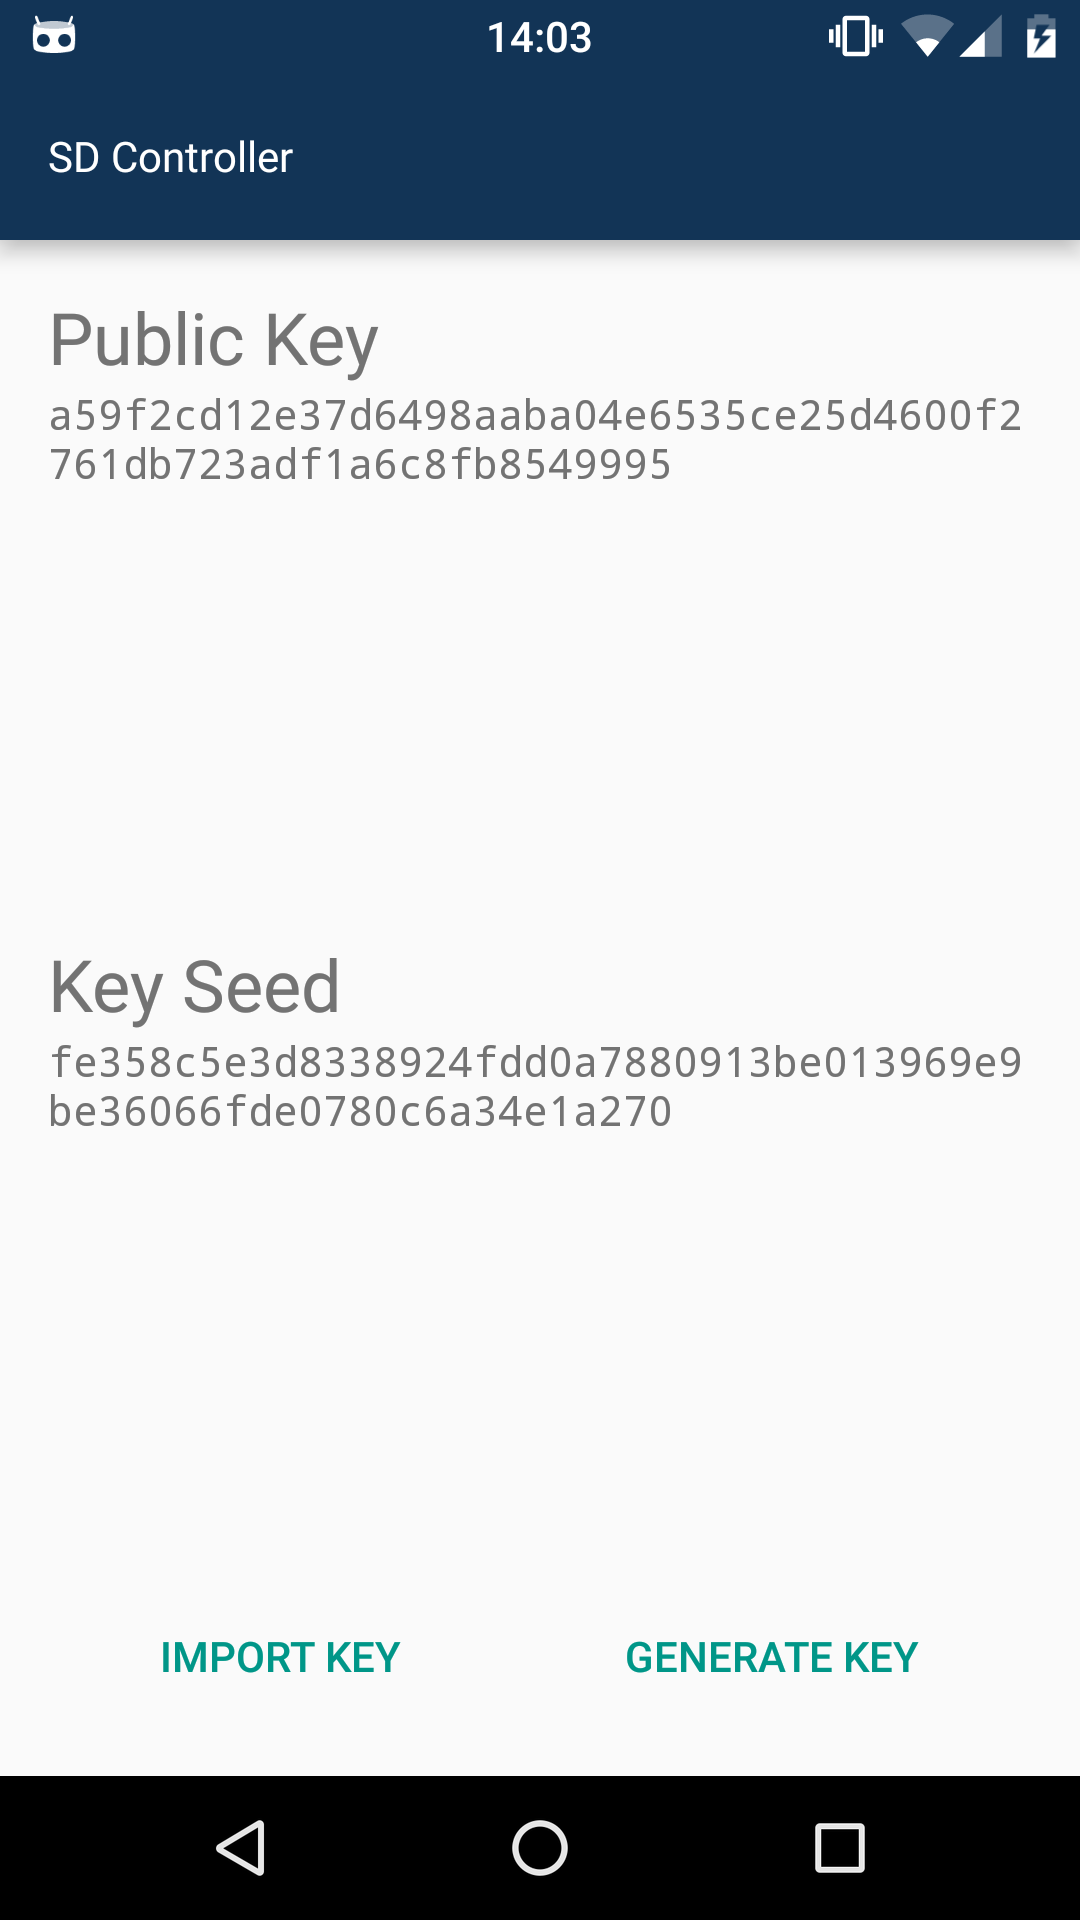
\includegraphics[width=\linewidth]{resources/identity.png}
        \caption{Identity}
        \label{identity}
    \end{subfigure}
    \begin{subfigure}{0.24\textwidth}
        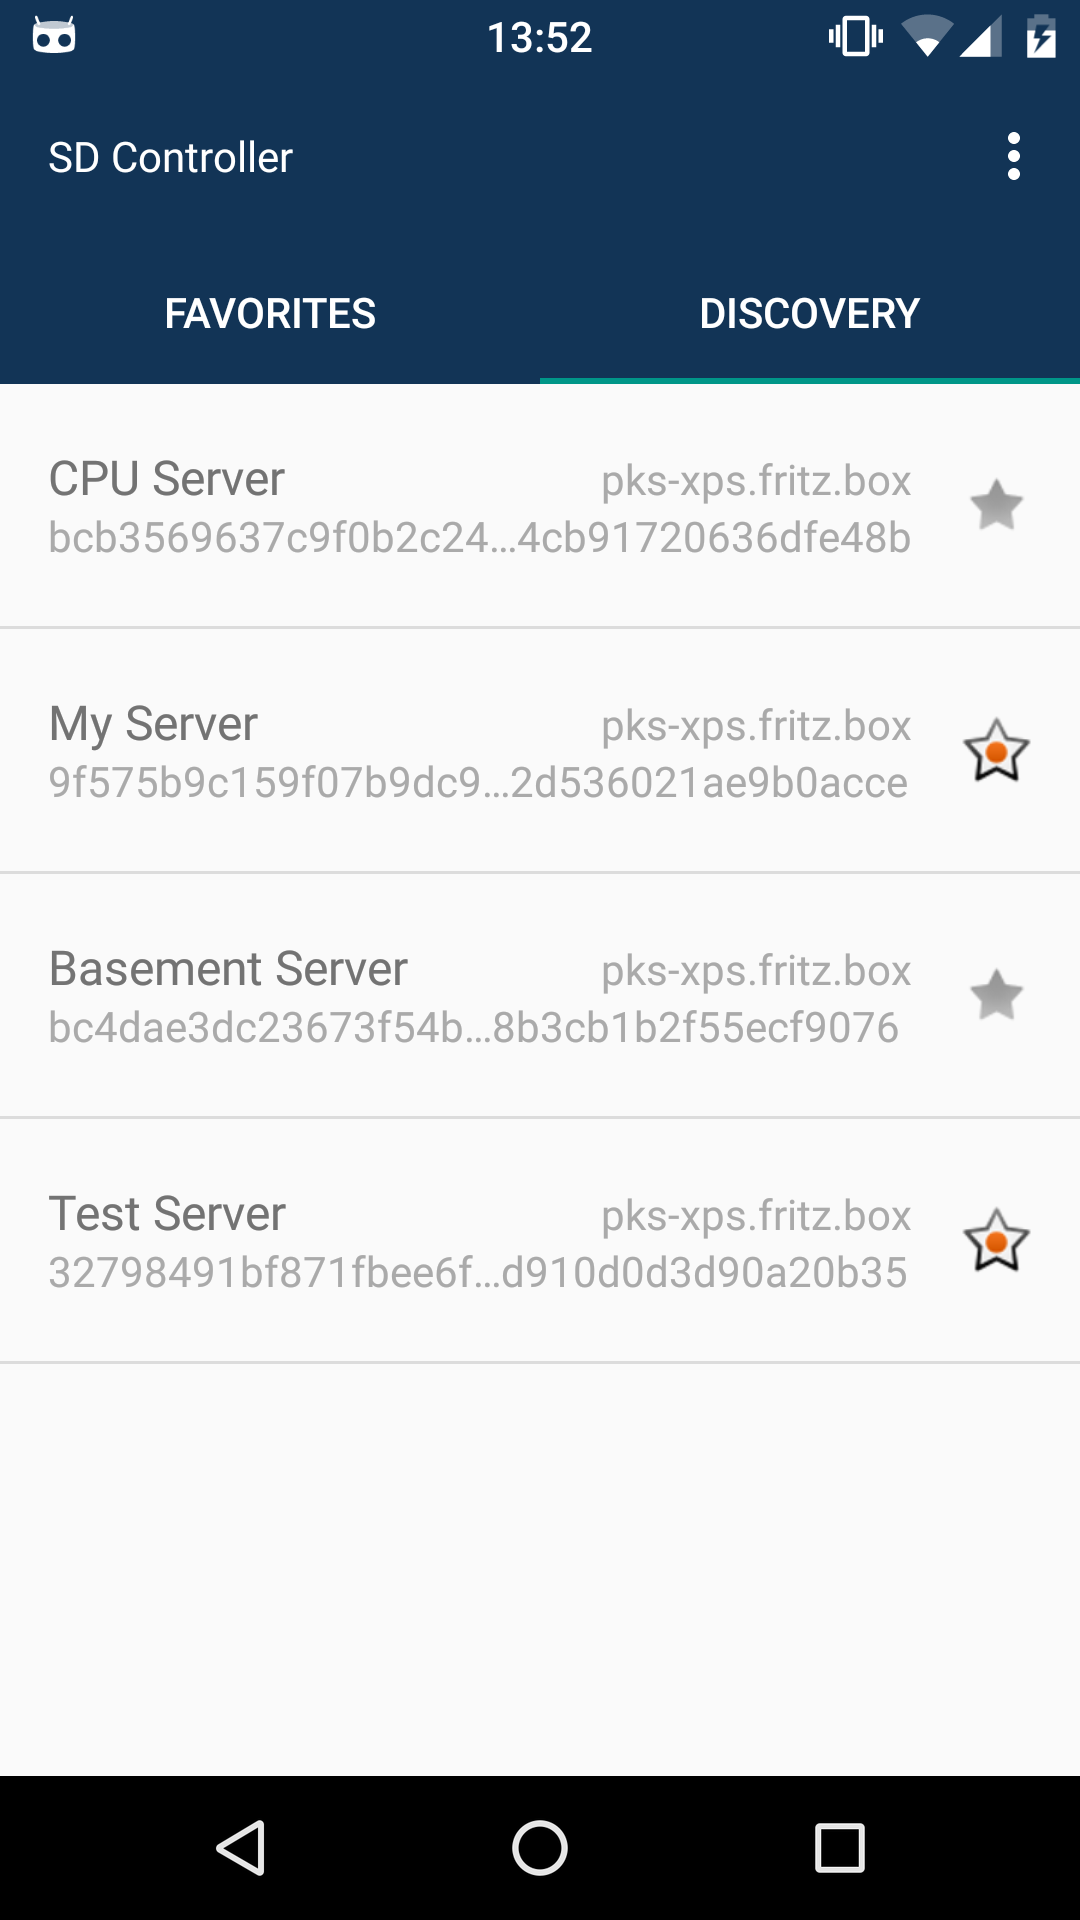
\includegraphics[width=\linewidth]{resources/discovery-list.png}
        \caption{Discovery list}
        \label{discovery-list}
    \end{subfigure}
    \begin{subfigure}{0.24\textwidth}
        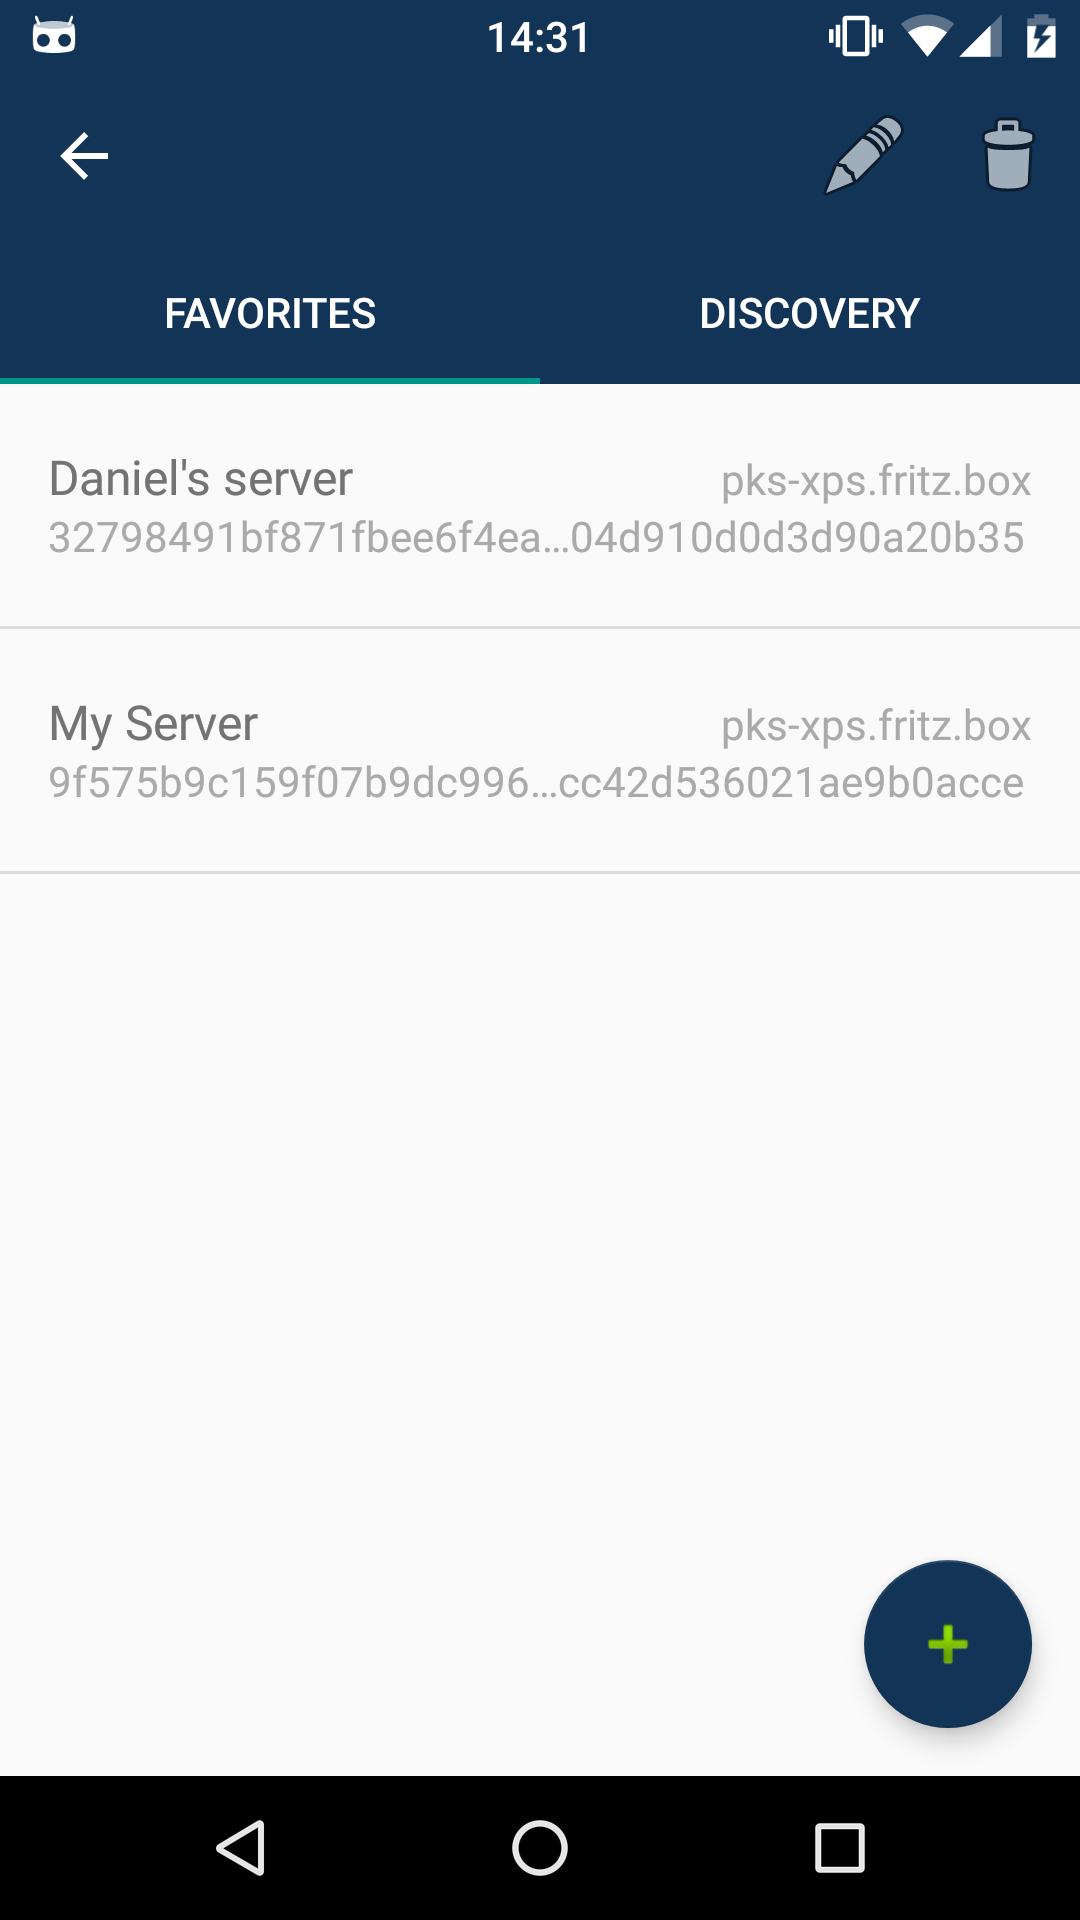
\includegraphics[width=\linewidth]{resources/favorites.png}
        \caption{Favorites list}
        \label{favorites-list}
    \end{subfigure}
    \begin{subfigure}{0.24\textwidth}
        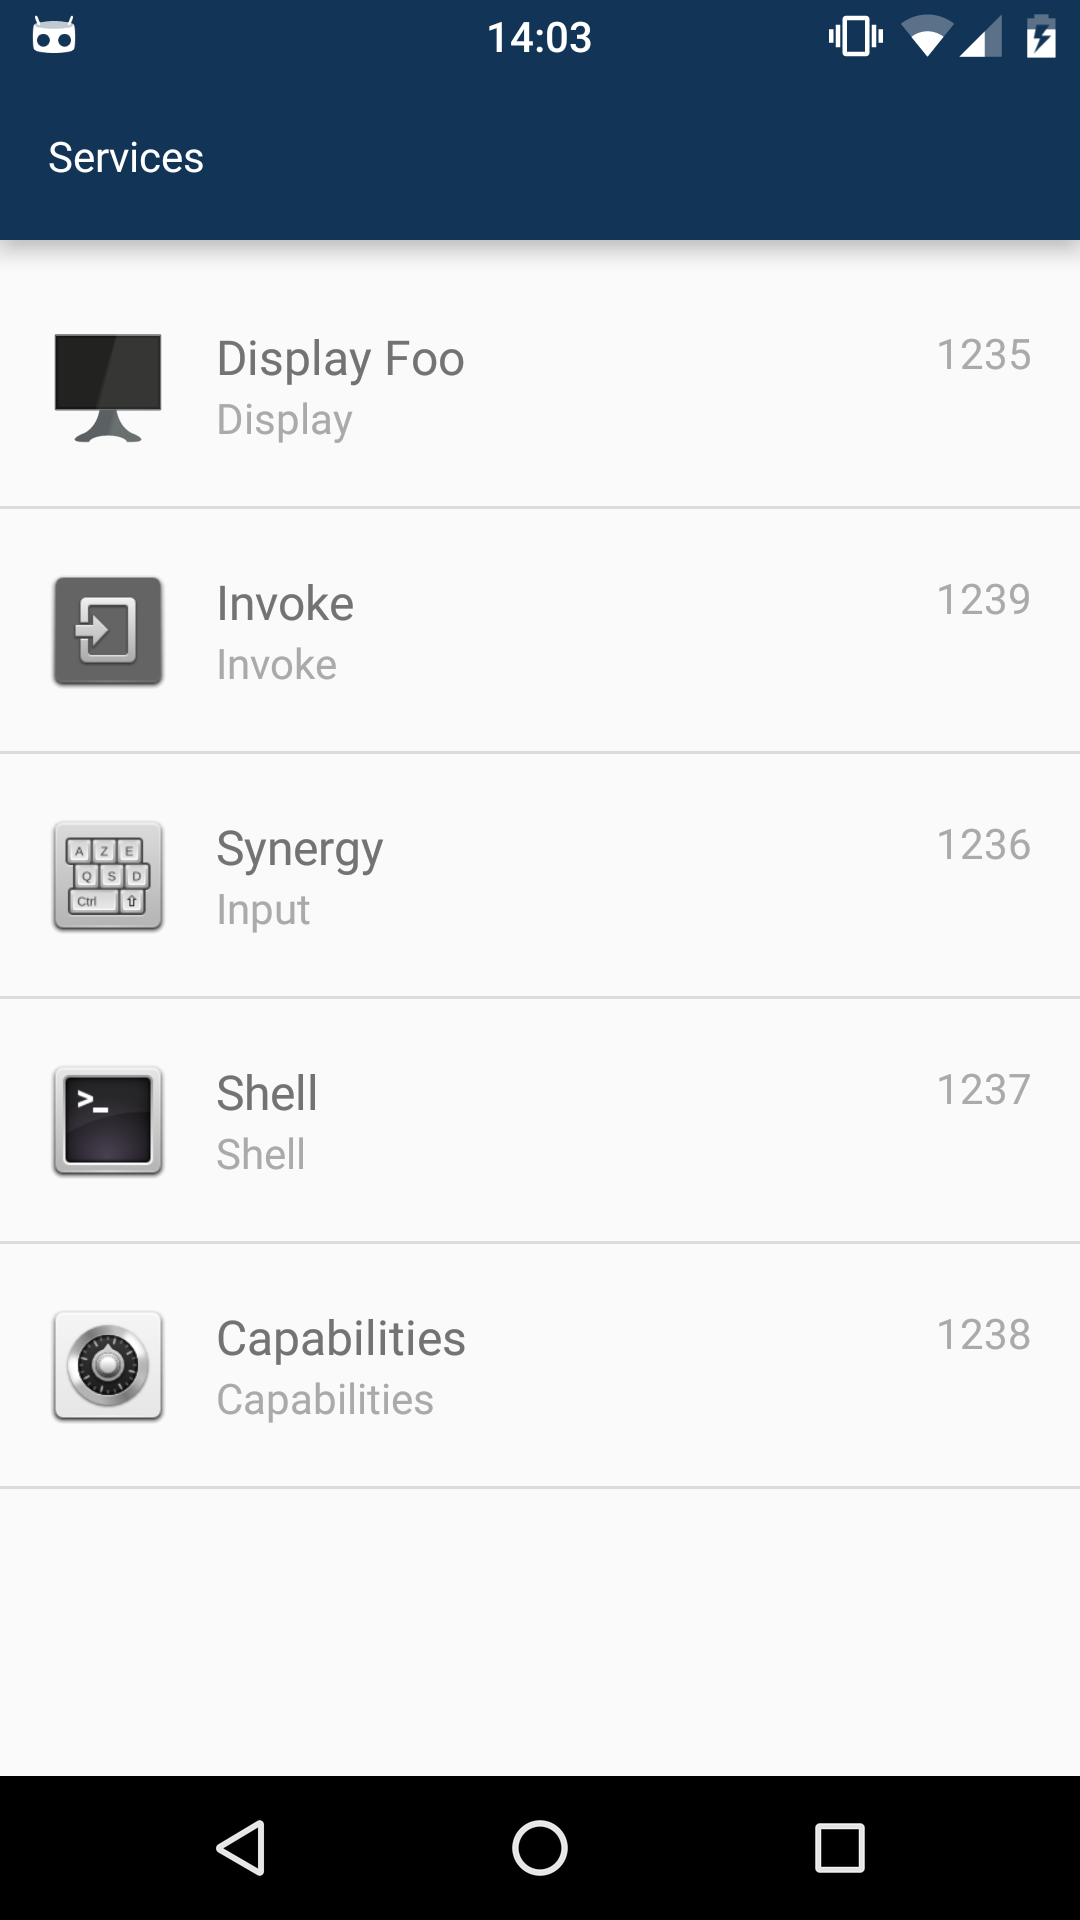
\includegraphics[width=\linewidth]{resources/services-list.png}
        \caption{Services list}
        \label{services-list}
    \end{subfigure}

    \caption{Android controller views}
\end{figure}

The current user interface presented to achieve this is rather simple.
Upon startup, the user gets presented a tabbed layout, where one of these tabs represents the user's favorite servers with which the user has already paired before, and the other tab is used to discover new services.
The initial step performed by users is to either generate a new key, which is automatically done on first startup of the application, or to import a previously generated key which is already known to other services.
This is done in the application's identity screen, depicted in figure \ref{identity}, which is accessible via the hamburger menu from the application's initial screen (the three dots in the upper right corner in figure \ref{discovery-list}).

One problem that spans through the complete Android application is the representation of key material.
Simply displaying the hexadecimal encoding of these keys, like it is currently displayed, is problematic as these strings are not easily recognizable for users.
Especially in the case where public keys are displayed for servers, it is especially hard to verify a server's identity is really the one we expect a server to have.
Assuming an adversary hosting a server in the local network, he may try to generate a key pair whose public key has only a small Levenshtein distance.

One paper discussing this issue is \cite{perrig1999hash}.
They observe that humans are inherently unreliable at comparing keys with each other, as these are only meaningless concatenations of symbols.
To fix the problem, they propose to instead display \emph{random art} derived from a hash of the public key instead, as humans are more reliable at recognizing previously seen images instead of recognizing random strings.
One project where random art is used to display keys is OpenSSH \cite{ylonen1996ssh} in the form of ASCII art.
Given that the application is a proof-of-concept only, no such solution has been implemented yet.

When the user has set up his key pair, he may now want to actually use the application and connect to services.
When the mobile client has not been previously paired with a server providing a certain service the user wants to connect with, he will choose the service discovery tab, upon which the application will start the discovery protocol to detect present servers.
For each server that is found, a new entry will be added to the list (see figure \ref{discovery-list}).
Each entry has displayed the server's name, its network address, an excerpt from its public key as well as a favorite-button.
The favorite button is displayed as a star, which is either displayed in color, indicating that the server has been saved to the user's favorites, or grayed out.
By tapping the button, users can add or remove the server from the favorites list.

This state helps the user to identify services which he already knows.
Furthermore, favorite servers may have a different name chosen by the user himself.
Announce messages from the server include the server's name, which is chosen by the server's administrator.
When users want to more easily distinguish specific servers, they can change a server's name to a custom name.
This name will then be displayed in the favorites list, but also in the service discovery list.

When a server has been added to the favorites, it will be displayed in the favorites list (see figure \ref{favorites-list}).
This list essentially presents the same information as the discovery list for each server, barring the button which allows users to add services to as a favorite.
Following the user interface pattern of editing list items, a user can long-tap a single list item in order to enable action mode, in which the application's title bar will change to an action bar.
This action bar currently has two buttons for either removing the entry or renaming it, which is displayed in the screenshot.

The favorites list also has the functionality to add a custom server by tapping the $+$-button.
The user is then presented a dialog which asks him for a server address, the server's public key as well as a custom chosen name for the server.
So in case it is impossible to detect servers by service discovery, e.g. because the server is not connected to the local network, users can manually add these servers and interact with them, given they have a publicly accessible internet address.

On either selecting a server in the favorite's list or discovery list, all services provided by the server are displayed (see figure \ref{services-list}).
For each service, we display its name as chosen by the server administrator, the service's category (e.g. ``Display'' or ``Input''), its port as well as an image, representing the service's functionality.
This image shall guide users to more easily distinguish available services.

When the user now wants to connect of one of these services presented, he will simply tap on the corresponding list item and an interface will be presented which gives access to the service's specific parameters.
E.g. given a shell service, the user will be presented fields to input an executable as well as its arguments and environment variables.
Having selected the parameters, he will now click on the ``Invoke'' button and gets presented a window showing the command's output.

Each service type has its own specific layout for presenting parameters.
One of the more important services for mobile clients is the ``Invoke'' service:
It allows a mobile client to connect two servers with each other, for example to connect the user's CPU server located in his office with the display in the conference room.
Upon selecting the Invoke service, he will be asked for a service which should be invoked from the server where the Invoke service is hosted.
Assuming the Invoke service is hosted on his office's work station, he simply directs it to invoke the display service located at the confercence room and tap ``Invoke'', upon which both servers connect to each other.

In the future, it might also be desirable to have some services which are able to operate with the mobile client itself instead of requiring a second server.
One of these services might be an input service, where the user is able to steer a display's mouse cursor as well as its keyboard by using the mobile client itself.

\bigskip

One problem with mobile clients is that they are inherently less safe than servers located at ones home or in datacenters.
It is much easier to loose or have stolen a mobile phone or tablet than to loose a full desktop computer.
Even when the device has full disk encryption enabled, unlocking the contents is usually only a 4-digit pincode away.
Due to this consideration, many a user does not want to store highly sensitive data like his long-term signature key on the device.

Fortunately, the protocol allows for the scenario where the mobile client is not required to know the actual long-term signature key but still connect to service requiring this key, required the user has access to a trusted server.
The setup required is similar to the setup presented in section \ref{sec:kerberos} on Kerberos.
Given the long-term signature key of the mobile client, which is distinct from the user's actual long-term signature key, he sets up a capability server on his home server.
Connected to the capability server is a simple policy client which grants all session requests from the mobile client's public signature key.
The policy client has access to the actual key pair and will use it for requesting the desired sessions.

So whenever the mobile client wishes access to a service in the name of his actual long-term signature key, he will simply request the capability service to request a new session with his actual key.
The policy client will accept the request when it is the mobile client's key, create a new session for the required service and forward the session to the mobile client.
The mobile client may now use the session.

Like this, only a single instance is required to know the actual key.
This instance shall obviously be protected so that no person has access to it and may extract the key.
Still, loss of the key is much harder than loss when the key is distributed to several clients, including mobile clients.

% vim: ft=tex tw=0
